\chapter{Case Studies}

%short introduction
%one section for each one of the case studies
%general structure for each one of the sections
    %1) Description of the model with Event-B code
    %2) Results of the simulation

The purpose of these case studies is to test the correct integration of the encoder with the MultiVeStA tool. In total there are 3 case studies: two probabilistic programs using dices and coins, a bounded re-transmission protocol, and a program that simulates a modal operator in positive negative logic. The repository that contains the code of this integration can be found in the following repository: \url{https://github.com/dfosorio/EventB2Maude-MultiVeStA}. Furthermore, this repository contains the code of the probabilistic Event-B models, their translated versions in PMaude, and the results of the simulations of the case studies. A short guide on how to use the software can also be found in the repository, for any reader that might want use the tool.



\section{Dice Programs}
The dice programs, based on the Knuth \& Yao paper \cite{knuth}, were originally discovered in the PRISM model checker web page \cite{PRISMDICE}. The idea is then to translate the model from the PRISM language to probabilistic Event-B, and afterwards translate the probabilistic Event-B model into PMaude using the encoder. The resulting PMaude specification will then be verified using MultiVeStA. If the results from the MultiVeStA simulations are the same as the PRISM model checker, then we can assume that the encoding and verification process were performed correctly. The probabilistic model for the first dice program is the following:
\begin{figure}[H]
    \centering
    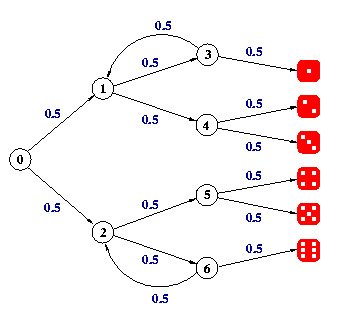
\includegraphics[scale = 0.5]{images/CS1.png}
    \caption{States and transitions of the dice model, taken from \cite{PRISMDICE}}
    \label{fig:ce1}
\end{figure}
Having as a reference the Figure \ref{fig:ce1}, the starting state of the model is the state 0. A fair coin is tossed to decide the next transition to execute. If the coin lands on heads, then the upper branch is taken. Conversely, when the coin lands on tails, the lower branch is taken. This process is repeated in each on of the sates 1 to 6, until reaching a terminating state, i.e. reaching a state where one of the dice faces is chosen. To represent this model in probabilistic Event-B, a deferred set with all the states of the model is created in the context.
\begin{maude}

CONTEXT ctxDiceProgram1
SETS 
    STATES : { s0, s1, s2, s3, s4, s5, s6, s7 }
CONSTANTS 
END
\end{maude}
where the state $s_7$ represents all the possible terminating states. In the machine of the model, two variables will be considered: one that stores the current state of the system and other that contains the current value of the dice.
\begin{maude}

MACHINE DiceProgram1
  SEES ctxDiceProgram1
  
  VARIABLES
    st 
    dice 
  INVARIANTS
    st : STATES
    dice : Nat 
\end{maude}
Each one of the transitions or coin tosses is represented with an event. For example, the first two transitions that start in state 0 can be represented with the event:
\begin{maude}

EVENT State0Trans 
WEIGHT 1
WHERE 
    st = s0
THEN
    st := {s1 @ 0.5 , s2 @ 0.5 }
END
\end{maude}
As seen in the event, the fifty-fifty probability of the coin toss is represented with a probabilistic assignment. For transitions that precede a terminating state, they are represented by changing the state to $s_7$, and assigning to the dice the respective value. For example, the transitions that branch out of the fourth state are represented in Event-B as:
\begin{maude}

EVENT State4Trans 
WEIGHT 1
WHERE 
    st = s4
THEN
    st := s7
    dice := {2 @ 0.5 , 3 @ 0.5 }
END    
\end{maude}
Finally, to initilize the system the values $s_0$ and 0 are assigned to the variables $st$ and $dice$ respectively.
\begin{maude}

INITIALISATION
    st := s0
    dice := 0
\end{maude}


The property that wants to be verified for this program is the probability of reaching a terminating state where the value of $dice = k$, where $k = 1,2,...,6$. if the model is correct, then the probability is $P(dice = k) = \frac{1}{6}$ for all $k$.

Using the encoder, the PMaude specification is obtained by repeating the process in Chapter 3. The file that contains this specification can be found in the repository with the filename \texttt{DiceProgram1.maude}. In order to define the user observations \texttt{rval}, an equation needs to be added that obtains the value of the dice variable. Therefore, for each one of the possible values of the dice (1 to 6) an equation is added that returns true (represented as 1.0 since \texttt{rval} return float numbers) if the dice has that specific value. For example, to verify that the dice has the value 1, the following equation is added to the PMaude specification:
\begin{maude}

  --- User Defined Observations 
eq val("obs1",{Conf < MNAME:Machine | 
                    variables:('st |-> st , 'dice |-> dice) >} 
                    {gt | SL}) 
                    = toFloat(((dice) =b (val(elt(1))))) .
\end{maude}
Hence, when the \texttt{s.rval("obs1")} is called in the MultiQuaTEx file, it will return 1.0 if the value of the dice is 1, and 0.0 otherwise. Moreover, for every encoded model, the encoder will also generate inside the specification two equations that can be used to define \texttt{rval} observations, regarding the terminating state of the model:
\begin{maude}

eq val("isMax", {Conf} {gt | SL}) = if (gt >= MAX-STEPS) 
                                    then 1.0 
                                    else 0.0 fi .

 eq val("deadlock", {Conf < events : Events | state: (LEv) >} 
                    {gt | SL}) = if (not-unknown(LEv) and 
                                    not(one-firable(LEv))) 
                                 then 1.0 
                                 else 0.0 fi .
\end{maude}
The first equation returns 1.0 (true) if the maximum number of transitions have been exeuted. Each transition corresponds to the execution of the $chooseEvt$ rule, and the number that defines the maximum number of transitions is specified as a constant named as \texttt{MAX-STEPS} in the specification. By default it is set to 10000, but it can be modified directly in the PMaude specification. Inside the specification, this number is used to bound the number of transitions of the PMaude model, and terminating its execution when the number is reached.

The second equation returns 1.0 if the model has reached a deadlock, i.e. none of the guards of the translated events have been satisfied. To do this, the equation \texttt{not-unknown} (it verifies that all the states have a state different from \texttt{unknown}) and \texttt{one-firable} (it verifies if there is at least one event with satisfied guards) are used. It is important to understand correctly these two equations, since they will be used to define the terminating condition of most of the PMaude specifications that result from the translation. 

For the verification of the model, the MultiQuaTEx formula that is used to verify the model is:
\begin{maude2}

PDice1(n) = if ((s.rval("isMax") == 1.0) || (s.rval("deadlock") == 1.0)) 
            then s.rval(n) else # PDice1(n) fi ;

eval E[ PDice1("obs1") ] ;
eval E[ PDice1("obs2") ] ;
eval E[ PDice1("obs3") ] ;
eval E[ PDice1("obs4") ] ;
eval E[ PDice1("obs5") ] ;
eval E[ PDice1("obs6") ] ;
\end{maude2}
When a terminating state is reached, i.e. the simulation reached the maximum number of transitions or the simulation reached a deadlock state, then the formula returns the the value of the observation \texttt{s.rval(n)} where \texttt{n} is a parameter of the formula, that is going to be replaced in each one of the evaluation calls with \texttt{"obs1"},\texttt{"obs2"}... or \texttt{"obs6"}. Using this formula, and the parameters $\alpha = 0.01, \delta = 0.01$ and $bs = 28$, the results of the simulation using MultiVeStA where:
\begin{table}[H]
\centering
\begin{tabular}{|l|l|l|l|}
\hline
Property     & ObtainedValue     & Variance          & CI                  \\ \hline
PDice1(obs1) & 0.169194084235345 & 0.140571212336999 & 0.00999772484533201 \\ \hline
PDice1(obs2) & 0.165127336320909 & 0.137864066309953 & 0.00999898248710578 \\ \hline
PDice1(obs3) & 0.166322650733297 & 0.138663192561158 & 0.00999737034957979 \\ \hline
PDice1(obs4) & 0.164898271712973 & 0.137710597576251 & 0.00999724079076279 \\ \hline
PDice1(obs5) & 0.166095890410959 & 0.138511810325858 & 0.00999571303811207 \\ \hline
PDice1(obs6) & 0.167870619946092 & 0.139693840237627 & 0.00999651791545913 \\ \hline
\end{tabular}
\end{table}

\begin{figure}[H]
    \centering
    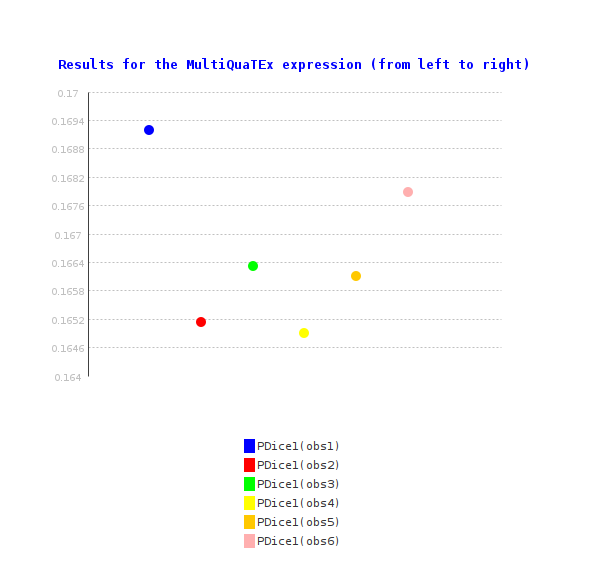
\includegraphics[scale = 0.5]{images/CS2.png}
    \caption{Graph of the simulation results of the first dice program}
    \label{fig:ce2}
\end{figure}
The number of simulations performed to obtain the results were 37324, and the time it took to run them was 2521.757 seconds (42 minutes). From this simulation, it is safe to say that the obtained results are close to the expected real value of $\frac{1}{6}$.

The second dice program corresponds to the same scenario, but considering two dice throws, i.e. the same transition system but simulated twice. This time, the property that wants to be verified is the probability of obtaining $k$ as the sum of the results of both dice, where $k = 2,3,4,...,12$. The expected probability for each one of the possible sums of two dice is:

\begin{table}[H]
\centering
\begin{tabular}{|l|l|l}
\cline{1-2}
k  & Probability &  \\ \cline{1-2}
2  & 1/36        &  \\ \cline{1-2}
3  & 1/18        &  \\ \cline{1-2}
4  & 3/36        &  \\ \cline{1-2}
5  & 1/9         &  \\ \cline{1-2}
6  & 5/36        &  \\ \cline{1-2}
7  & 1/6         &  \\ \cline{1-2}
8  & 5/36        &  \\ \cline{1-2}
9  & 1/9         &  \\ \cline{1-2}
10 & 3/36        &  \\ \cline{1-2}
11 & 1/18        &  \\ \cline{1-2}
12 & 1/36        &  \\ \cline{1-2}
\end{tabular}
\end{table}
To specify the model, one approach would be to add new variables \textit{state2}, \textit{dice2}, and duplicate the events specified in the previous dice program to change the new variables. Event though implementing the Event-B model in this way would work, for this model the optimized version proposed in \cite{knuth} will be used. This version consists of the same principle: multiple states and coin tosses as transitions, until reaching a terminating state, i.e. the sum of two dices. The graph that represents this model is:
\begin{figure}[H]
    \centering
    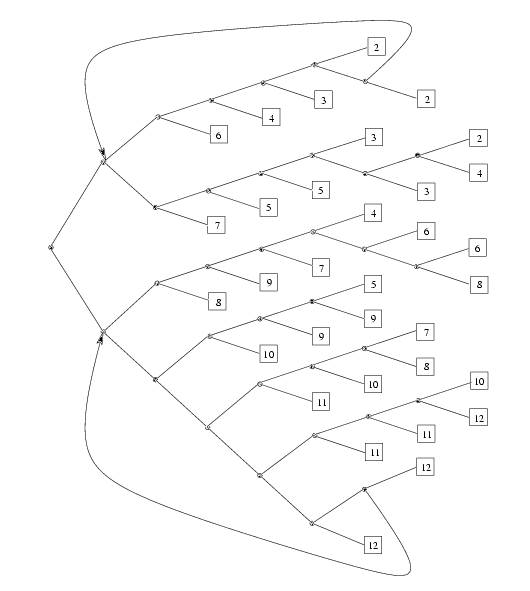
\includegraphics[scale=0.4]{images/CS3.png}
    \caption{States and transitions of the two dice model, taken from \cite{PRISMDICE}}
    \label{fig:ce3}
\end{figure}
Each one of the nodes in Figure \ref{fig:ce3}, represents a state in the probabilistic Event-B model. Therefore, the new context is going to specify a deffered set with 33 states, and an extra 34th state to specify a terminating state.
\begin{maude}

CONTEXT ctxDiceProgram2
SETS 
    STATES : { s0, s1, ... , s33, s34 }
CONSTANTS 
END
\end{maude}
For the variables, and the initialization of the machine, the Event-B specification is identical. Finally, for the events of the model the principle is the same: For each one the transitions use a probabilistic assignment to symbolize the fifty-fifty chance in the system transitions. The resulting probabilistic Event-B model and the encoded version in PMaude, can be consulted in the \texttt{DiceProgram2.b} and \texttt{DiceProgram2.maude} files respectively. The equations that define the user observations are also defined in the same manner:
\begin{maude}

eq val("obs1", {Conf < MNAME : Machine | 
                     variables: ('st |-> st , 'diceSum |-> diceSum) >} 
                     {gt | SL}  ) = toFloat(((diceSum) =b (val(elt(2))))) .
\end{maude}
In this case \texttt{"obs1"} references the case where $k = 2$, \texttt{"obs2"} references the case $k = 3$, and so on until \texttt{"obs11"}. The MultiQuaTEx formula used to verify the model is also very similar to the previous one:
\begin{maude2}

PDice2(n) = if ((s.rval("isMax") == 1.0) || (s.rval("deadlock") == 1.0)) 
            then s.rval(n) else # PDice2(n) fi ;

eval E[ PDice2("obs1") ] ;
eval E[ PDice2("obs2") ] ;
eval E[ PDice2("obs3") ] ;
eval E[ PDice2("obs4") ] ;
eval E[ PDice2("obs5") ] ;
eval E[ PDice2("obs6") ] ;
eval E[ PDice2("obs7") ] ;
eval E[ PDice2("obs8") ] ;
eval E[ PDice2("obs9") ] ;
eval E[ PDice2("obs10") ] ;
eval E[ PDice2("obs11") ] ;
\end{maude2}
Using this formula, and the parameters $\alpha = 0.01, \delta = 0.01$ and $bs = 100$, the results of the simulation using MultiVeStA where:

\begin{table}[H]
\centering
\begin{tabular}{|l|l|l|l|}
\hline
Property      & ObtainedValue      & Variance           & CI                  \\ \hline
PDice2(obs1)  & 0.03               & 0.0291037312475958 & 0.00995116917577923 \\ \hline
PDice2(obs2)  & 0.0510077519379845 & 0.0484097138712153 & 0.00997972279089514 \\ \hline
PDice2(obs3)  & 0.0853365384615385 & 0.0780579664517895 & 0.00997985024064457 \\ \hline
PDice2(obs4)  & 0.114200743494424  & 0.101162694374703  & 0.00999035979240436 \\ \hline
PDice2(obs5)  & 0.138710691823899  & 0.119473792835145  & 0.00998550057004364 \\ \hline
PDice2(obs6)  & 0.164328767123288  & 0.137328585846037  & 0.00999266014168248 \\ \hline
PDice2(obs7)  & 0.135176848874598  & 0.116907827497064  & 0.00998823325270086 \\ \hline
PDice2(obs8)  & 0.110306513409962  & 0.0981427467677965 & 0.0099897800415653  \\ \hline
PDice2(obs9)  & 0.0811616161616162 & 0.0745781747981354 & 0.00999816628115168 \\ \hline
PDice2(obs10) & 0.0551798561151079 & 0.0521387905863524 & 0.00997746359029961 \\ \hline
PDice2(obs11) & 0.0282191780821918 & 0.0274266131408506 & 0.0099855441351178  \\ \hline
\end{tabular}
\end{table}

\begin{figure}[H]
    \centering
    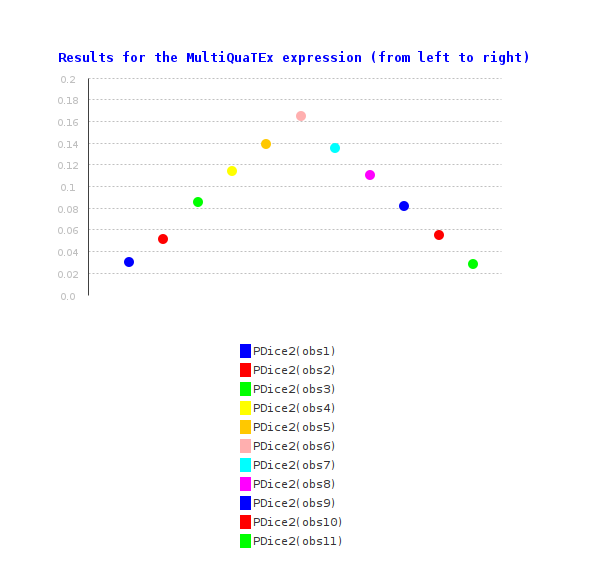
\includegraphics[scale = 0.5]{images/CS4.png}
    \caption{Graph of the simulation results of the second dice program}
    \label{fig:ce4}
\end{figure}
In total, the number of simulations performed to obtain the results were 36500, and the time it took to run them was 4583.059 seconds (76 minutes). In the end, the results of the simulation are very close to the expected probability for each one of the possible values of the sum of the two dice.

\section{Bounded Re-transmission Protocol}
The bounded re-transmission protocol is based on the sixth refinement of the file transfer protocol in Chapter six of Abrial's book \cite{Abrial2011}. In this occasion, a short explanation of the model will be given to understand the general intuition behind its behavior. The reader can refer to the explanation given in the book, or the model specification in the file \texttt{b-retrans-5.b} in the repository for further details. 

The file transfer protocol consists of a sender and a receiver, where the sender shares to the receiver a file. As seen in Figure \ref{fig:cs5}, there are two channels two ensure the communication between the sender and the receiver: the first one is the \textit{data channel}, used by the sender to transfer the file to the receiver, and the second one is the \textit{acknowledge channel}, used by the receiver to inform to the sender that the information that it has send, has already been received by the receiver.
\begin{figure}[H]
    \centering
    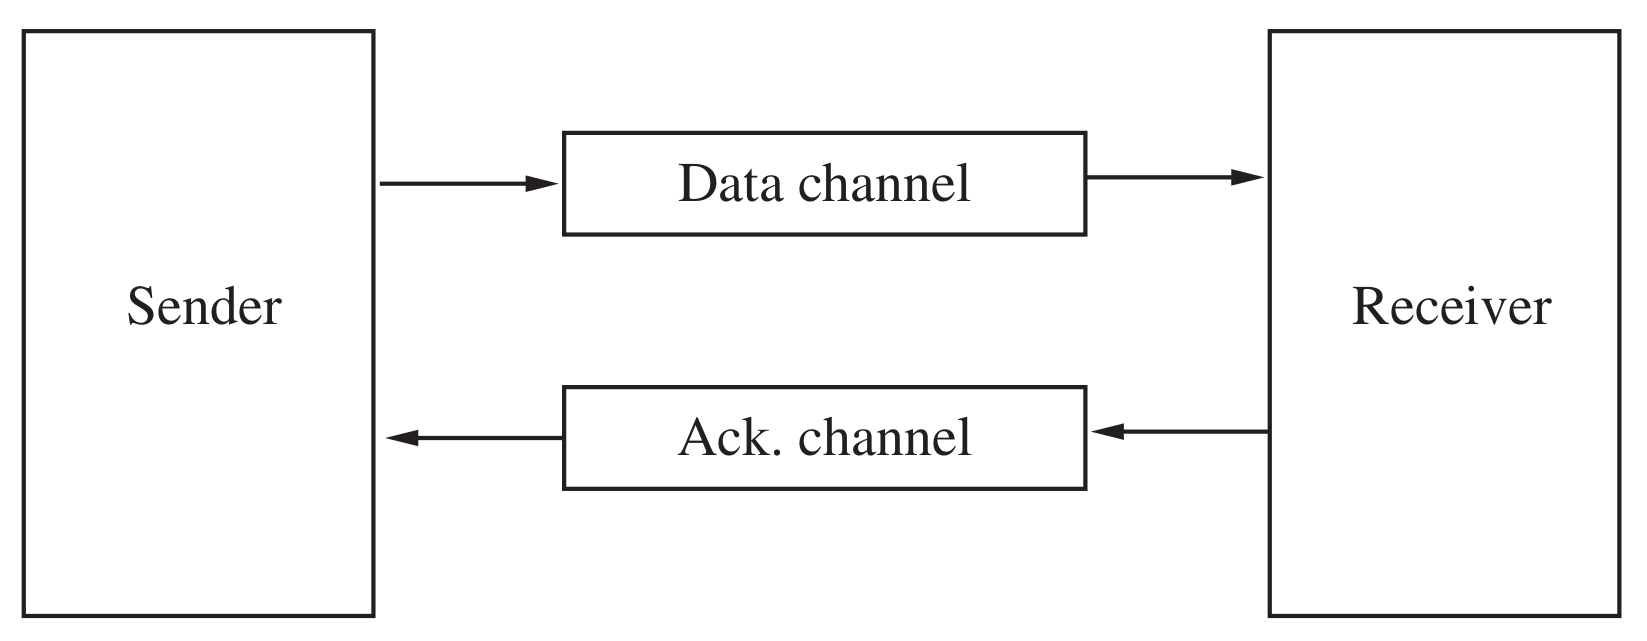
\includegraphics[scale = 0.2]{images/CS5.png}
    \caption{Interaction between sender and receiver, taken from \cite{Abrial2011}}
    \label{fig:cs5}
\end{figure}
The file can be considered as an array of values. Therefore, sending data to the receiver consists of sending one by one, through the data channel, the elements of the array as seen in Figure \ref{fig:cs6}  
\begin{figure}[H]
    \centering
    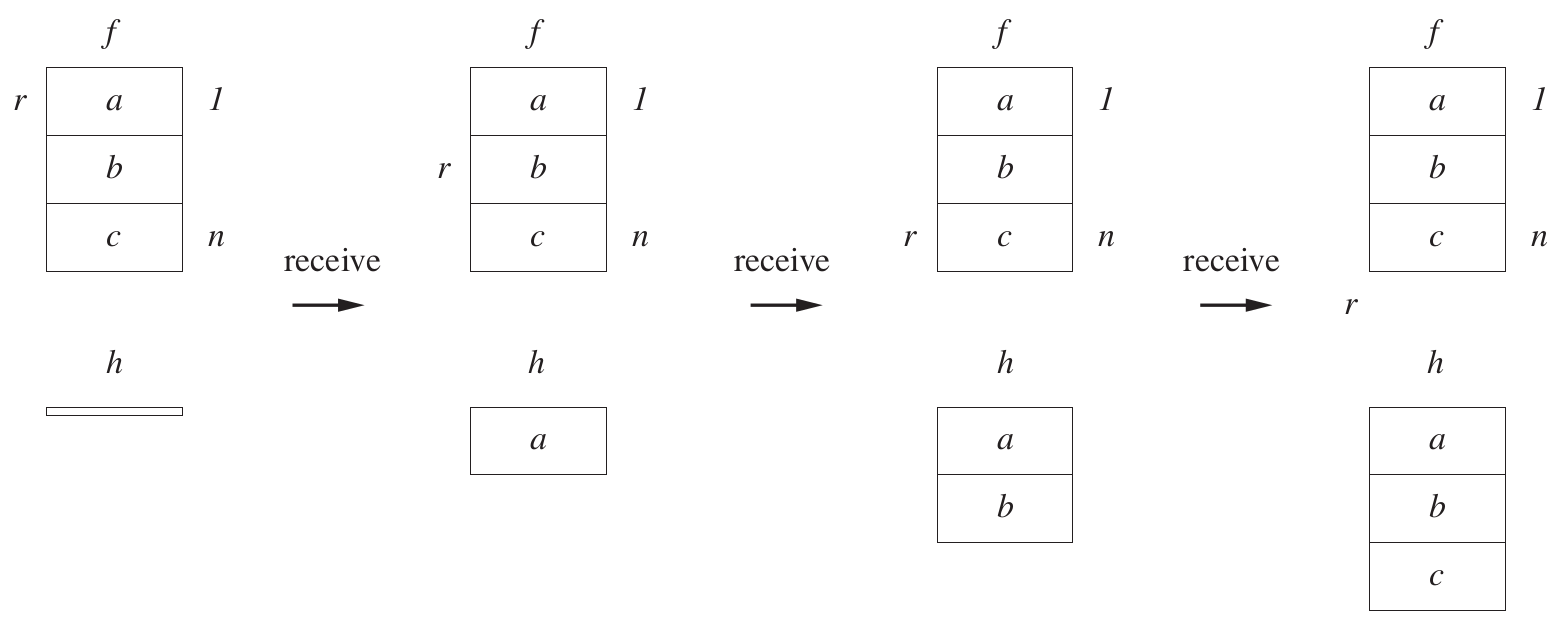
\includegraphics[scale = 0.3]{images/CS6.png}
    \caption{File transmission process from the sender to the receiver, taken from \cite{Abrial2011}}
    \label{fig:cs6}
\end{figure}
The protocol is completed when all the elements from the file have been transferred to the receiver, therefore reaching the success state. If the complete process is represented as a series of steps, the resulting list is:
\begin{enumerate}
    \item Initialize the system, i.e. initialize the file in the senders memory and other necessary variables for the transmission process.
    \item The sender sends the first element of the file.
    \item The receiver receives the sent element and returns to the sender the acknowledge signal.
    \item The sender receives the acknowledge signal.
    \item Steps 2, 3 and 4 are repeated with the following element, until sending all the elements of the file to the receiver. In that case, the system enters the success state, and the procedure is finished.
\end{enumerate}
The complete process can be visualized in Figure \ref{fig:cs7}:
\begin{figure}[H]
    \centering
    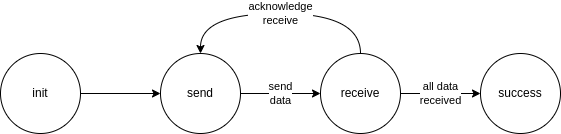
\includegraphics[scale = 0.7]{images/CS7.png}
    \caption{Complete file transmission process}
    \label{fig:cs7}
\end{figure}
Now, lets consider a model where both the data and acknowledge channel are unreliable, i.e. there exists the possibility of data loss when the file is sent, or when the acknowledgment message is sent. When this occurs, the protocol must retry to send the lost information. However, including a retry procedure can cause infinite loops in the system, since there exists a path in the model's transition where the system could send, fail and retry infinitely. To avoid this, a new constant is included in the system, named \textit{MAX}, that specifies the maximum number of retries that the protocol can make. If the maximum number of retries is exceeded then the protocol reaches the failure state, meaning that the file was not completely sent to the receiver. The complete process can be viewed in Figure \ref{fig:cs8}:     
\begin{figure}[H]
    \centering
    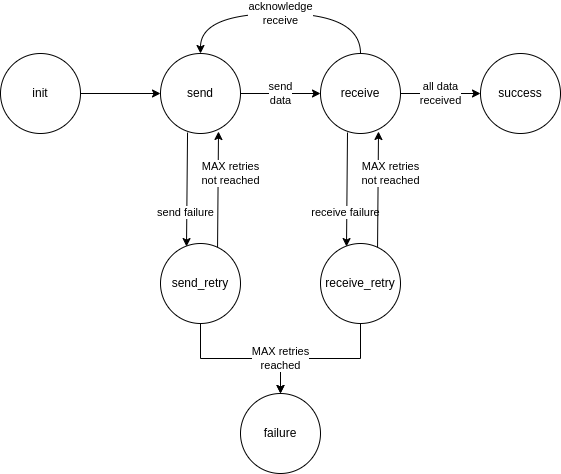
\includegraphics[scale = 0.6]{images/CS8.png}
    \caption{File transmission process with unreliable channels}
    \label{fig:cs8}
\end{figure}
In order to assign probabilities to the previously explained model, every time the sender or the receiver send information to one another, there is a $50\%$ chance of failure. Inside the \texttt{b-retrans-5.b} file, this behavior can be specified by assigning the same weight to the events that specify the action of sending successfully the message, and the events that specify the failure in the communication channels. Hence, the weight assigned to all the events is 1.

Given this probabilistic model, the property that wants to be verified using MultiVeStA is the probability of reaching the success state, using the maximum number of retries \textit{MAX}, as a parameter of the model. Thus, using the encoder, the \texttt{b-retrans-5.b} model was translated into PMaude. The user defined observations where:
\begin{itemize}
    \item \textbf{``obs1":} returns 1.0 if the state of the system is failed, and 0.0 otherwise.
    \item \textbf{``obs2":} returns 1.0 if the state of the system is success, and 0.0 otherwise.
\end{itemize}
And the MultiQuaTEx formula used to verify the model was:
\begin{maude2}

PRetrans5(n) = if ((s.rval("deadlock") == 1.0) || (s.rval("isMax") == 1.0)) 
               then s.rval(n) else # PRetrans5(n) fi ;

eval E[ PRetrans5("obs1") ] ;
eval E[ PRetrans5("obs2") ] ;
\end{maude2}

It states that when the system reaches a terminating state, i.e. reaching the failure or success state, since both of these states mean that the system enters a deadlock, then the formula verifies if the state of the system is successful or failed.
Using this formula, parameters $\alpha = 0.01, \delta = 0.01$, $bs = 100$, a fixed size for the file $N = 100$, and multiple values for the maximum number of retries $MAX$, the results of the simulation where:

% Please add the following required packages to your document preamble:
% \usepackage{multirow}
\begin{table}[H]
\centering
\resizebox{\columnwidth}{!}{
\begin{tabular}{|l|l|l|l|l|l|l|l|}
\hline
File size            & \textit{MAX}        & Simulations            & Time in seconds            & Property        & ObtainedValue      & Variance           & CI                  \\ \hline
\multirow{2}{*}{100} & \multirow{2}{*}{0}  & \multirow{2}{*}{100}   & \multirow{2}{*}{7.96}      & PRetrans5(obs1) & 1                  & 0                  & 0                   \\ \cline{5-8} 
                     &                     &                        &                            & PRetrans5(obs2) & 0                  & 0                  & 0                   \\ \hline
\multirow{2}{*}{100} & \multirow{2}{*}{5}  & \multirow{2}{*}{100}   & \multirow{2}{*}{19.633}    & PRetrans5(obs1) & 1                  & 0                  & 0                   \\ \cline{5-8} 
                     &                     &                        &                            & PRetrans5(obs2) & 0                  & 0                  & 0                   \\ \hline
\multirow{2}{*}{100} & \multirow{2}{*}{10} & \multirow{2}{*}{4200}  & \multirow{2}{*}{4695.782}  & PRetrans5(obs1) & 0.984285714285714  & 0.0154710305174701 & 0.0098873988006215  \\ \cline{5-8} 
                     &                     &                        &                            & PRetrans5(obs2) & 0.0154761904761905 & 0.0152403066489754 & 0.00981339506242592 \\ \hline
\multirow{2}{*}{100} & \multirow{2}{*}{15} & \multirow{2}{*}{13200} & \multirow{2}{*}{49320.0}   & PRetrans5(obs1) & 0.636742424242424  & 0.231319033581516  & 0.0215658109731058  \\ \cline{5-8} 
                     &                     &                        &                            & PRetrans5(obs2) & 0.359772727272727  & 0.230353763026125  & 0.0215207679775556  \\ \hline
\multirow{2}{*}{100} & \multirow{2}{*}{20} & \multirow{2}{*}{8900}  & \multirow{2}{*}{51120.0}   & PRetrans5(obs1) & 0.212111111111111  & 0.167138558605277  & 0.0222005711076664  \\ \cline{5-8} 
                     &                     &                        &                            & PRetrans5(obs2) & 0.786111111111111  & 0.168159116445037  & 0.0222682469512274  \\ \hline
\multirow{2}{*}{100} & \multirow{2}{*}{25} & \multirow{2}{*}{7700}  & \multirow{2}{*}{49560.0}   & PRetrans5(obs1) & 0.0507792207792208 & 0.0482069521594135 & 0.0128901078154959  \\ \cline{5-8} 
                     &                     &                        &                            & PRetrans5(obs2) & 0.949090909090909  & 0.0483236311681564 & 0.0129056978494018  \\ \hline
\multirow{2}{*}{100} & \multirow{2}{*}{30} & \multirow{2}{*}{2800}  & \multirow{2}{*}{19700.462} & PRetrans5(obs1) & 0.0103571428571429 & 0.0102535344255602 & 0.00985836415788304 \\ \cline{5-8} 
                     &                     &                        &                            & PRetrans5(obs2) & 0.989642857142857  & 0.0102535344255602 & 0.00985836415788304 \\ \hline
\end{tabular}
}
\end{table}

\begin{figure}[H]
    \centering
    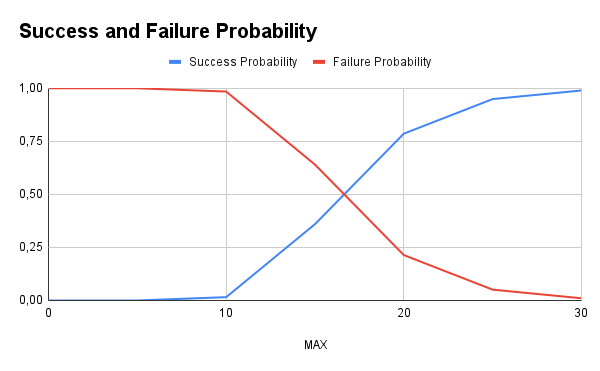
\includegraphics[scale = 0.5]{images/CS9.png}
    \caption{Graph of success and failure probability of the bounded re-transmission protocol}
    \label{fig:cs9}
\end{figure}

As seen in both the result table and the graph in Figure \ref{fig:cs9}, the probability of success is directly proportional to the maximum number of retries. Conversely, the probability of failure is inversely proportional to the maximum number of retries. This is the expected behavior, since incrementing the maximum number of retries of the protocol should increase the probability that the file is sent completely. It is important to note, that not all of the simulations reached the desired confidence interval ($CI < 0.01$). The reason behind this, is that the time it  was taking to reach the desired confidence interval was overly long, as seen in the previous table. Hence, some of the simulations were stopped before reaching the desired confidence interval. Nevertheless, the obtained confidence interval for the stopped simulations is good enough (approximately $CI < 0.023$) to approximate the probability of reaching a success or failure state.

\section{Balance Property in Signed Frames}
Positive negative logic or \textit{PNL} is a modal logic for Kripke structures introduced in \cite{PNL1, PNL2}, used to define properties over a specific class of network. For the moment, this section will only focus on the \textit{signed frame} structure and a dynamic model that modifies signed frames. The reader is encouraged to read the cited articles to understand the syntax, semantics and extension of PNL. Continuing then with the explanation, in these networks the nodes represent agents, and the connections or edges between them represent if two agents share the same or contrary opinion of a particular topic. Formally speaking, a network is represented as a signed frame of the form $\mathbb{F} = \langle A, R^+, R^- \rangle$, where $A$ is a set of agents, and $R^+,R^-$ are reflexive binary relations from $A$ to $A$. For any agent $a,b \in A$, if $(a,b) \in R^+$ then it means that agents $a$ and $b$ share the same opinion. Conversely, if $(a,b) \in R^-$, then $a$ and $b$ have different opinions. For example, lets consider the signed frame:
\begin{align*}
    \mathbb{F} = \langle \{a,b,c,d\}, \{(a,c),(b,d)\},\{(a,b),(a,d), (b,c)\} \rangle
\end{align*}
Graphically, this signed frame is represented by the graph:
\begin{figure}[H]
    \centering
    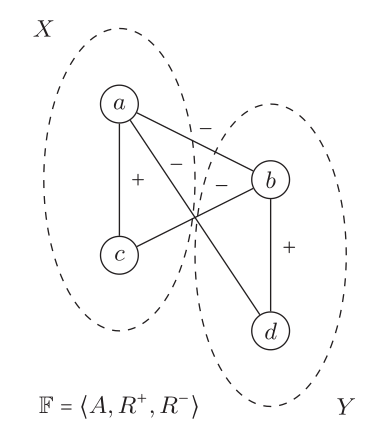
\includegraphics[scale = 0.5]{images/CS10.png}
    \caption{Graph that represents the signed frame $\mathbb{F}$, taken from \cite{PNL1}}
    \label{fig:CS10}
\end{figure}
One of the important properties that define these type of graph is the balance property. In short, a signed frame $\mathbb{F}$ is said to have the balance property, if $\forall a,b,c \in A$:
\begin{itemize}
    \item if $aR^+b$ and $bR^+c$, or $aR^-b$ and $bR^-c$, then $aR^+c$ and
    \item if $aR^+b$ and $bR^-  c$, or $aR^-b$ and $bR^+c$, then $aR^-c$.
\end{itemize}
The balance property is important since it allows to define group polarization in networks: when a network has the balance property, it is possible divide the set $A$ in two subsets $S$ and $A \setminus S$, where all the agents in the same subset share the same opinion, and agents from different subset have different opinion. In more detail, if $aR^+b$ then $a,b \in S$ or $a,b \in A \setminus S$. Moreover, if $aR^-b$ then $a \in S$ and $b \in A \setminus S$, or $b \in S$ and $a \in A \setminus S$. As an example, the signed frame in figure \ref{fig:CS10} has the balance property, and can be divided in two opposing groups $X$ and $Y$.

One of the extensions proposed to PNL in the article \cite{PNL1}, are the modalities $\langle \bigdoublewedge +\rangle$ and $\langle \bigdoublewedge - \rangle$, which can be explained as adding a positive and negative link somewhere in the network. One way to represent the previously explained behavior, is with a dynamic system that takes an initial signed frame, and non-deterministically adds positive and negative links until reaching a terminating state, i.e. all the links between the nodes of the graph have been added.

\begin{figure}[H]
    \centering
    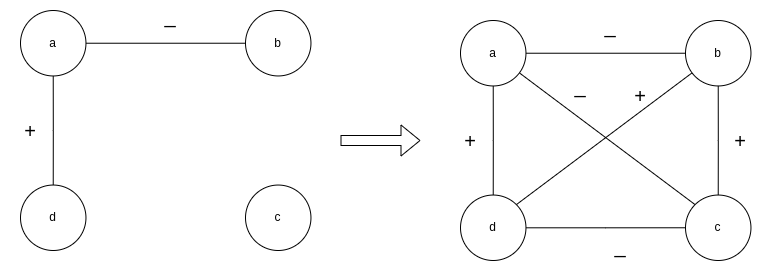
\includegraphics[scale=0.5]{images/CS11.png}
    \caption{Initial and possible terminating state of a simulation of the dynamic system.}
    \label{fig:CS11}
\end{figure}

To exemplify, if the graph in the left side of Figure \ref{fig:CS11} is considered as the initial state of the dynamic system, then one of the possible outcomes of the simulation, after adding non-deterministically positive and negative links, is the graph in the right side of Figure \ref{fig:CS11}. The idea is then to elaborate a probabilistic Event-B model that has the same behavior as described before. The probability of the system lies on the choice of adding a positive or negative link. In this case, the probability for both actions will be fifty percent. Therefore, the context of the model would contain the set of all the agents in the signed frame. For example, if $A = \{a,b,c\}$ then the context would be:
\begin{maude2}

CONTEXT ctxPNL
SETS 
    AGENTS : { a, b, c } # nodes of the graph #
CONSTANTS 
END
\end{maude2}

For the machine 3 variables will be used: two relations that represent the relations $R^+$ and $R^-$ of the signed frame, and an extra variable that contains all the possible edges of the signed frame, which will remain constant throughout the complete simulation and will be used to identify the missing edges to add to the graph.

\begin{maude2}

MACHINE PNL
  SEES ctxPNL

  VARIABLES
    AgentsComb # set of all possible edges #
    Rpositive # relation that represents positive edges in graph #
    Rnegative # relation that represents negative edges in graph # 

  INVARIANTS
    Rpositive :  POW ( AGENTS ** AGENTS )
    Rnegative :  POW ( AGENTS ** AGENTS )
    AgentsComb :  POW ( AGENTS ** AGENTS )
\end{maude2}
The action of adding positive and negative edges to the graph is represented with two events that have the same weight, thus giving to each one of the events a fifty percent probability of occurring. 
\begin{maude2}

  EVENT addPositiveEdge 
  WEIGHT 1
  ANY 
    edge <: (AgentsComb \ Rpositive) \ Rnegative
  WHERE
    True 
  THEN
    Rpositive := Rpositive \s/ edge
  END

  EVENT addNegativeEdge 
  WEIGHT 1
  ANY 
    edge <: (AgentsComb \ Rpositive) \ Rnegative
  WHERE
    True 
  THEN
    Rnegative := Rnegative \s/ edge
  END
\end{maude2}
The initialization event depends of the initial configuration of the signed frame. For example, if the signed frame has the form of the graph on the right of figure \ref{fig:CS11}, the initialization event would be:
\begin{maude2}
    
INITIALISATION
    AgentsComb := { a |-> b, a |-> c, a |-> d, 
                    b |-> c, b |-> d,
                    c |-> d }
    Rpositive := {a |-> d} 
    Rnegative := {a |-> b}
\end{maude2}

Based on this probabilistic Event-B model, the property that wants to be verified is: given an initial configuration for a signed frame, what is the probability of reaching a terminating state where the signed frame has the balance property. To complete the task, three different experiments with three signed frames will be run using the encoder and MultiVeStA. The first experiment corresponds to the following signed frame:
\begin{figure}[H]
    \centering
    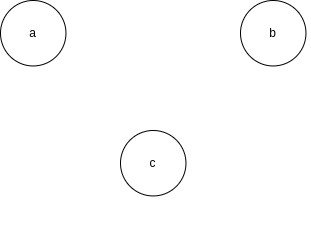
\includegraphics[scale=0.5]{images/CS13.png}
    \caption{Signed frame of the first experiment}
    \label{fig:CS13}
\end{figure}
In total, there are four out of eight possible configurations, where the resulting signed frame is balanced.
\begin{table}[H]
\centering
        \begin{tabular}{lccc|c|}
        \cline{2-5}
        \multicolumn{1}{l|}{} & \multicolumn{1}{c|}{(a,b)} & \multicolumn{1}{c|}{(a,c)} & (b,c)                 & Balanced \\ \cline{2-5} 
        \multicolumn{1}{l|}{} & \multicolumn{1}{c|}{+}     & \multicolumn{1}{c|}{+}     & +                     & yes      \\ \cline{2-5} 
        \multicolumn{1}{l|}{} & \multicolumn{1}{c|}{-}     & \multicolumn{1}{c|}{+}     & +                     & no       \\ \cline{2-5} 
        \multicolumn{1}{l|}{} & \multicolumn{1}{c|}{+}     & \multicolumn{1}{c|}{-}     & +                     & no       \\ \cline{2-5} 
        \multicolumn{1}{l|}{} & \multicolumn{1}{c|}{+}     & \multicolumn{1}{c|}{+}     & -                     & no       \\ \cline{2-5} 
        \multicolumn{1}{l|}{} & \multicolumn{1}{c|}{-}     & \multicolumn{1}{c|}{-}     & +                     & yes      \\ \cline{2-5} 
        \multicolumn{1}{l|}{} & \multicolumn{1}{c|}{-}     & \multicolumn{1}{c|}{+}     & -                     & yes      \\ \cline{2-5} 
        \multicolumn{1}{l|}{} & \multicolumn{1}{c|}{+}     & \multicolumn{1}{c|}{-}     & -                     & yes      \\ \cline{2-5} 
        \multicolumn{1}{l|}{} & \multicolumn{1}{c|}{-}     & \multicolumn{1}{c|}{-}     & -                     & no       \\ \cline{2-5} 
                              & \multicolumn{1}{l}{}       & \multicolumn{1}{l}{}       & \multicolumn{1}{l|}{} & 50\%     \\ \cline{5-5} 
        \end{tabular}
        \end{table}
It is then expected that the results obtained by the MultiQuaTEx formula is near the $\frac{1}{2}$ value. After translating the probabilistic Event-B model to a Maude specification, a user defined equation is added to the specification. The equation \texttt{Balanced} takes as input
the current state of the signed frame, i.e. the value of relations $R^+$ and $R^-$, and checks if the signed frame is balanced. If it is balanced, then it returns 1.0 and 0.0 otherwise. To verify that the signed frame is balanced, the equation verifies if all the triangles in the signed frame satisfy the balance property. For more detail, the reader can refer to the \texttt{PNL1.maude} file for more information on the implementation of the equation. Lastly, the MultiQuaTEx formula used to verify the property is defined as follows:
\begin{maude2}

PPNL(n) = if ((s.rval("isMax") == 1.0) || (s.rval("deadlock") == 1.0)) 
	     then s.rval(n) else # PPNL(n) fi ;

eval E[ PPNL("balanced") ] ; 
\end{maude2}

It states that when a terminating states is reached, then return the value of evaluating the \texttt{Balanced} equation over the last state. Using this formula, and the parameters $\alpha = 0.01, \delta = 0.01$ and $bs = 100$, the results of the simulation using MultiVeStA where:

\begin{table}[H]
\centering
\resizebox{\columnwidth}{!}{
\begin{tabular}{|l|l|l|l|l|l|}
\hline
Property       & Time in seconds & Simulations & ObtainedValue     & Variance          & CI                 \\ \hline
PPNL(balanced) & 2735.93         & 46400       & 0.497948164146868 & 0.250001189563359 & 0.0119709224484389 \\ \hline
\end{tabular}
}
\end{table}

As seen in the table, the obtained value for the formula is within the expected range of the real value. It is worth noting that the desired confidence interval with $\delta = 0.01$ was not reached since in the last MultiVeStA cycle, the returned value for the confidence interval was \texttt{NaN}, i.e. not a number. For the time being, the source of this behavior is unclear, but with the previously obtained values, it is possible to form an idea on the expected value for the query. The other two experiments correspond to the following signed frames:

\begin{figure}[H]
    \centering
    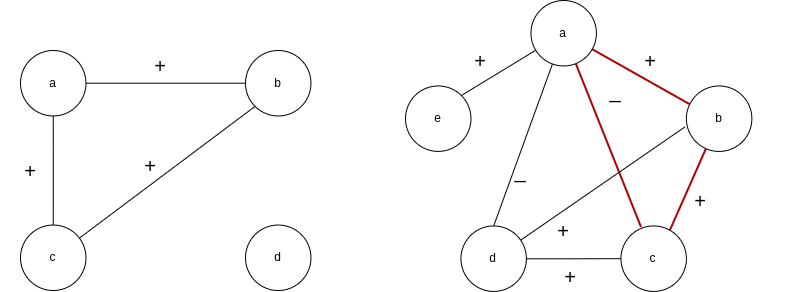
\includegraphics[scale = 0.5]{images/CS14.png}
    \caption{Signed frames of experiment 2 (left) and experiment 3 (right)}
    \label{fig:CS14}
\end{figure}

For the experiment 2 (left side of Figure \ref{fig:CS14}), the chances of reaching a terminating state that is balanced are two out of eight ($25\%$ chance), and for experiment 3 the probability is $0\%$, since the initial configuration already includes a triangle that is not balanced, which is highlighted in red. The MultiQuaTEx query used for both experiments is the same one as experiment 1, and the obtained results with parameters $\alpha = 0.01, \delta = 0.01$ and $bs = 100$ where: 
\begin{table}[H]
\centering
\resizebox{\columnwidth}{!}{
\begin{tabular}{|l|l|l|l|l|l|}
\hline
Experiment & Time in seconds & Simulations & ObtainedValue     & Variance          & CI                \\ \hline
1          & 2639.935        & 46400       & 0.254341252699784 & 0.189655876114114 & 0.010426528417539 \\ \hline
2          & 5.631           & 100         & 0                 & 0                 & 0                 \\ \hline
\end{tabular}
}
\end{table}

The results obtained in the simulations are in accordance with the real expected value of the queries. For the experiment 2, the \texttt{NaN} value was also obtained before reaching the desired confidence interval, therefore the estimation of the expected value of the query was done with the value obtained in the previous batch of simulations. Still, the confidence interval is good enough for an approximation of the expected value of the query.














    